\documentclass[a4paper,11pt]{article}

\usepackage{tecnico_relatorio}

\usepackage{textcomp}
\usepackage[hypcap]{caption} % makes \ref point to top of figures and tables
%\usepackage{rotating}
\usepackage{float}
\usepackage[nottoc]{tocbibind}
\usepackage[utf8]{inputenc}
\usepackage{graphicx}
\usepackage[justification=centering]{caption}
\usepackage{listings}
\usepackage{indentfirst} % indent first paragraph in section
\usepackage{geometry}	% margins


% magic for listings (make them beautiful)
\usepackage{color}
\usepackage{xcolor}

\definecolor{very-light-gray}{rgb}{0.95, 0.95, 0.95}
\DeclareCaptionFont{white}{\color{white}}
\DeclareCaptionFormat{listing}{\colorbox{gray}{\parbox{\textwidth}{#1#2#3}}}
\captionsetup[lstlisting]{format=listing, labelfont=white, textfont=white}
\lstset{backgroundcolor = \color{very-light-gray}, xleftmargin=7pt, frame=lr, framesep=7pt, framerule=0pt, breaklines=true, tabsize=4, showstringspaces=false}

  % a tab is 4 spaces
%\usepackage{fancyvrb}
%\fvset{tabsize=2}


\begin{document}
\newgeometry{left=4.0cm,right=4.0cm}

\trSetImage{img/tecnico_logo}{6cm} % Logotipo do Técnico

\trSetCourse{Mestrado em Engenharia Electrotécnica \\e de Computadores}

\trSetSubject{Sistemas de Informação e \\ Bases de Dados}

\trSetType{Part II}

\trSetTitle{Project Assignment}

\trSetBoxStyle{0.3}

\trSetGroupNo{Group 1}

\trSetAuthorNr{3}

\trSetAuthors
{
    \begin{center}
	Gonçalo Ribeiro

	73294
    \end{center}
}{
    \begin{center}
	Ricardo Amendoeira

	73373
    \end{center}
}{
    \begin{center}
	Rodrigo Veríssimo

	76971
    \end{center}
}

\trSetProfessor{Prof. José Alberto Sardinha}

\trMakeCover

\restoregeometry
\newgeometry{left=2.5cm,right=2.5cm}

\tableofcontents
\pagenumbering{gobble}

\pagebreak

\pagenumbering{arabic}
\setcounter{page}{1}



\section{Database creation}

\subsection{Database Schema}

The database is created according to the provided schema. The file that sets up the database is  called \texttt{databaseCreate.sql}. This file can be seen in \autoref{lst:databaseCreate}.

For textual columns we used the \texttt{varchar} type as it is a variable length type and therefore can result in smaller storage. \texttt{varchar} was also used to store devices' serial numbers so that they can be alphanumeric instead of being strictly numeric. The maximum length of each column was defined to values that we deemed reasonable.

Mobile numbers, municipality codes and patient IDs are created as \texttt{unsigned integer}s. On the other hand, values for readings and writings we used the \texttt{decimal} type.

To store dates the \texttt{datetime} type was used. This type allows us to store both the date and time on a single field.

All the primary and foreign keys were created as defined in the provided schema. The constraints introduced by these keys result in that the order of creation of the tables is not aribitrary. For example, the table \texttt{Actuator} has a foreign key to the \texttt{Device} table. Therefore, \texttt{Actuator} can only be created after the creation of \texttt{Device}. Creating the tables in an order that results in no errors is possible. But it is not desirable that the tables need to be created in a specific order. Therefore we used the \texttt{foreign\_key\_checks} MySQL option to disable the foreign key checking while doing the \texttt{drop}s and \texttt{create}s that set up the database. This way we could order both the \texttt{drop}s and \texttt{create}s alphabetically, which results in improved readability of the script. The use of \texttt{foreign\_key\_checks} can be seen in \autoref{lst:databaseCreate}.

At the end of the script the triggers and procedures are \texttt{source}d, so that the database is completely ready to be used when the script ends.


\lstinputlisting[language=SQL, label=lst:databaseCreate, caption=\texttt{databaseCreate.sql}]
{../databaseCreate.sql}

\subsection{Triggers}

The database is expected to fire an error whenever trying to connect a device or patient to a PAN for a period of time overlapping an existing period for that device or patient. To enforce this behaviour we create four triggers: two triggers \texttt{before insert} and other two \texttt{before update}. These triggers check if a period incompatible with the one we are trying to create exists. If it does, then an inexistent procedure \texttt{overlapping\_data()} is called. When this procedure is called an error will be generated (since the procedure does not exist) and this will rollback any changes that were made. 

One thing we thought about is that triggering an error by calling a non-existing procedure is not a clean way to go about it. If in the future a procedure was added to the database with the same name as the procedure that is called to generate the error then not only would an error not be generated but also the \texttt{insert}/\texttt{update} could work when it should not. As of MySQL 5.5 a new keyword \texttt{signal} exists that allows to ``\thinspace`return' an error''. This keyword also allows to set an error message.

Listings \ref{lst:triggerDeviceTimeOverlap} and \ref{lst:triggerUpdateDeviceTimeOverlap} show the triggers for inserting and updating a new device. The triggers for associating patients to a PAN are very alike the ones to associate devices (see Listings \ref{lst:triggerPatientTimeOverlap} and \ref{lst:triggerUpdatePatientTimeOverlap}).


\lstinputlisting[language=SQL, label=lst:triggerDeviceTimeOverlap, caption=\texttt{triggerDeviceTimeOverlap.sql}]{../triggerDeviceTimeOverlap.sql} 

\lstinputlisting[language=SQL, label=lst:triggerPatientTimeOverlap, caption=\texttt{triggerPatientTimeOverlap.sql}]{../triggerPatientTimeOverlap.sql} 

\lstinputlisting[language=SQL, label=lst:triggerUpdateDeviceTimeOverlap, caption=\texttt{triggerUpdateDeviceTimeOverlap.sql}]{../triggerUpdateDeviceTimeOverlap.sql}

\lstinputlisting[language=SQL, label=lst:triggerUpdatePatientTimeOverlap, caption=\texttt{triggerUpdatePatientTimeOverlap.sql}]{../triggerUpdatePatientTimeOverlap.sql} 


\pagebreak
\section{Queries}

In this section the queries written for Question 2 of the assignment are presented.

\subsection{Readings in the last 6 months concerning `blood pressure'}

\lstinputlisting[language=SQL, label=lst:queryReadings, caption=\texttt{queryReadings.sql}]{../queryReadings.sql}


%%%%%

\pagebreak
\subsection{Municipality with the highest number of devices from Philips}

\lstinputlisting[language=SQL, label=lst:queryMunicipality, caption=\texttt{queryMunicipality.sql}]{../queryMunicipality.sql}


%%%%%

\pagebreak
\subsection{Manufacturers that during the last year had a `scale' being worn in all municipalities}

\lstinputlisting[language=SQL, label=lst:queryManufacturer, caption=\texttt{queryManufacturer.sql}]{../queryManufacturer.sql}


%%%%%

\pagebreak
\section{The web application}

In this section the pages and the website frontend and backend are presented. The main application page can be seen in \autoref{img:index}.

\begin{figure}[h]
    \centering
    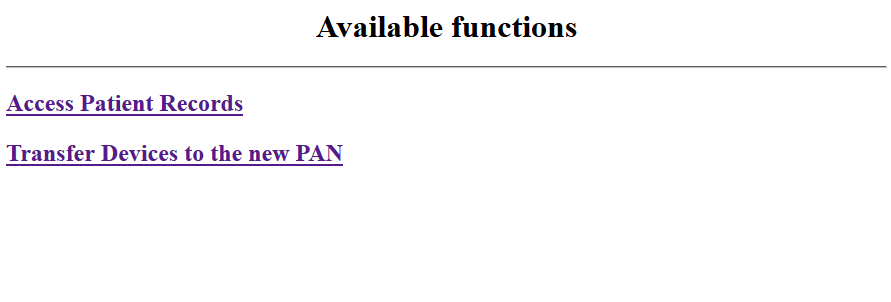
\includegraphics[width=.8\textwidth]{img/index}
    \caption{\texttt{index.php}}
    \label{img:index}
\end{figure}


\subsection{Search patients and show readings and settings}

\begin{figure}[h]
    \centering
    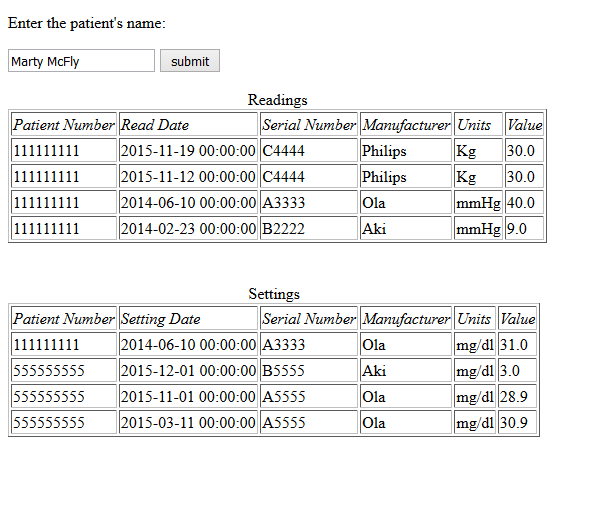
\includegraphics[width=.8\textwidth]{img/Registos}
    \caption{\texttt{patient\_records.php}}
    \label{img:patient_records}
\end{figure}

\lstinputlisting[language=PHP, label=lst:patient_records, caption=\texttt{patient\_records.php}]{../patient_records.php}

\lstinputlisting[language=SQL, label=lst:display_all_readings, caption=\texttt{display\_all\_readings.sql}]{../display_all_readings.sql}

\lstinputlisting[language=SQL, label=lst:display_all_settings, caption=\texttt{display\_all\_settings.sql}]{../display_all_settings.sql}


\pagebreak
\subsection{Transfering devices from a patients' old PAN to his new one}

\begin{figure}[h]
    \centering
    \centerline{
      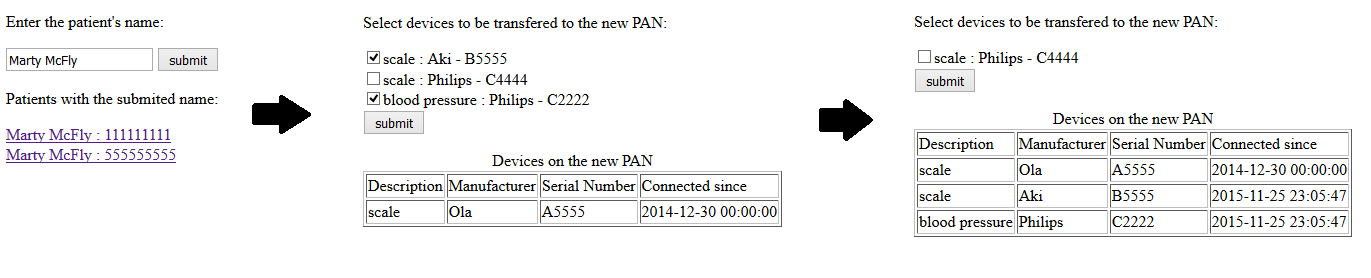
\includegraphics[width=\textwidth]{img/Transferir_all}
    }
    \caption{\texttt{transfer\_devices.php}}
    \label{img:transfer_devices.php}
\end{figure}

\lstinputlisting[language=PHP, label=lst:transfer_devices, caption=\texttt{transfer\_devices.php}]{../transfer_devices.php}

\lstinputlisting[language=PHP, label=lst:transfer_devices2, caption=\texttt{transfer\_devices2.php}]{../transfer_devices2.php}


\pagebreak
\appendix
\section{Sample data for the database}

The file in \autoref{lst:sampledata} was used to populate the database and do subsequent testing of the project's functionalities.

\lstinputlisting[language=SQL, label=lst:sampledata, caption=\texttt{testingdata/databaseInsert.sql}]{../testingdata/databaseInsert.sql}

\end{document}


%\lstinputlisting[language=, label=lst:, caption=\texttt{}]{../}


